\chapter{Performance Profiles}
These experiments are updated as of the current date: 8 February 2022.

I've made some experiments by inflating the vehicle capacity of the original CVRP instances.

Let $Q$ and $k$ denote respectively the CVRP instance vehicle capacity and the number of vehicles.
Define a scale factor $s \in \N$, a new CVRP instance is generated from the old one using pseudo algorithm steps:

\begin{align}
	Q \gets Q \times s \\
	k \gets \ceil*{\frac{k}{s}}
\end{align}

\renewcommand{\do}[1]{
	\begin{figure}[ht]
		\centering
		\begin{subfigure}{0.5\textwidth}
			\centering
			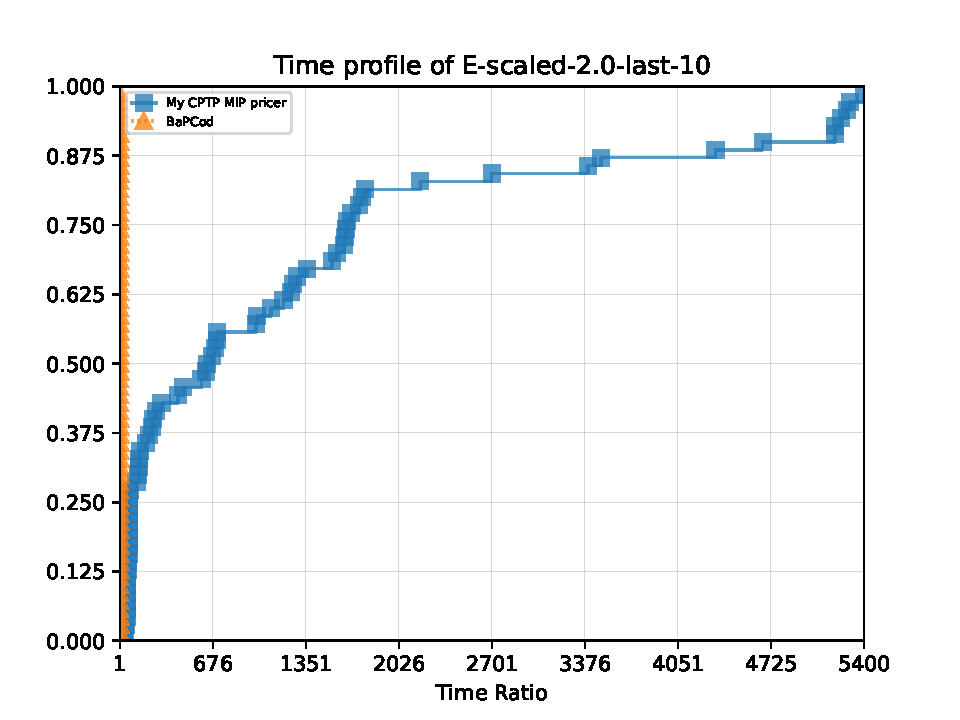
\includegraphics[width=1.0\linewidth]{#1/Time Ratio Plot.pdf}
		\end{subfigure}%
		\begin{subfigure}{0.5\textwidth}
			\centering
			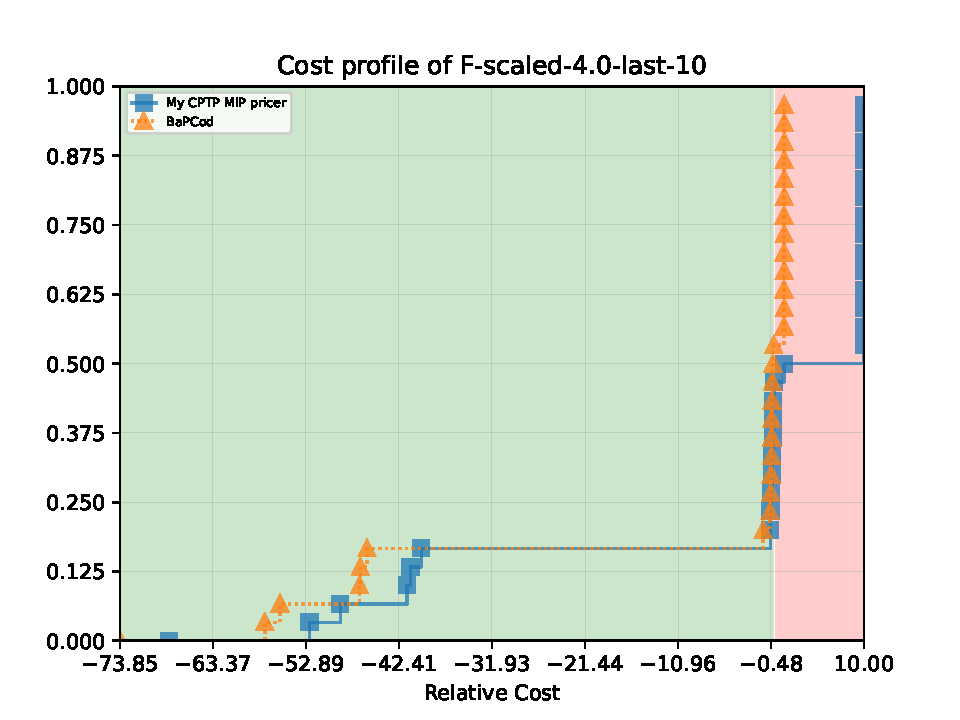
\includegraphics[width=1.0\linewidth]{#1/Relative Cost Plot.pdf}
		\end{subfigure}%
	\end{figure}
}

\docsvlist{Imgs/perfprofs/E-scaled-1.0-last-10}
\docsvlist{Imgs/perfprofs/E-scaled-2.0-last-10}
\docsvlist{Imgs/perfprofs/E-scaled-4.0-last-10}
\docsvlist{Imgs/perfprofs/F-scaled-1.0-last-10}
\docsvlist{Imgs/perfprofs/F-scaled-2.0-last-10}
\docsvlist{Imgs/perfprofs/F-scaled-4.0-last-10}
